\documentclass[xcolor=pdftex,dvipsnames,table]{beamer}
\usetheme{Boadilla}
\usecolortheme{seahorse}
\usepackage{etex}
\providecommand\thispdfpagelabel[1]{}
\usepackage{amsmath}
\usepackage{mathtools}
\usepackage{amssymb}
\usepackage{amsthm}
\usepackage{listings}
\usepackage{graphics}
\usepackage{framed}
\usepackage{etex}
\usepackage{tcolorbox}
\usepackage[all]{xy}
\usepackage{svg}
\usepackage{xspace,listings,ulem,tikz}
\usepackage[outline]{contour}
\usepackage[absolute,overlay]{textpos}
\usepackage{hhline}
\usepackage{pgffor}
\usepackage[square,sort,comma,numbers]{natbib}
\usepackage{CJKutf8}
\usetikzlibrary{tikzmark,fit,shapes.geometric}
 \setbeamertemplate{footline}{%
      \raisebox{5pt}{\makebox[\paperwidth]{\hfill\makebox[10pt]{\scriptsize\insertframenumber}}}}
\tikzset{
    onslide/.code args={<#1>#2}{% http://tex.stackexchange.com/a/6155/16595
        \only<#1>{\pgfkeysalso{#2}}
    },
    hideshow/.style args={<#1><#2>#3}{%
        onslide=<#1>{move to},
        onslide=<#2>{#3}
    }
}
\lstset{
         basicstyle=\footnotesize\ttfamily, % Standardschrift
         %numbers=left,               % Ort der Zeilennummern
         numberstyle=\tiny,          % Stil der Zeilennummern
         %stepnumber=2,               % Abstand zwischen den Zeilennummern
         numbersep=5pt,              % Abstand der Nummern zum Text
         tabsize=2,                  % Groesse von Tabs
         extendedchars=true,         %
         breaklines=true,            % Zeilen werden Umgebrochen
         keywordstyle=\color{red},
 %        keywordstyle=[1]\textbf,    % Stil der Keywords
 %        keywordstyle=[2]\textbf,    %
 %        keywordstyle=[3]\textbf,    %
 %        keywordstyle=[4]\textbf,   \sqrt{\sqrt{}} %
         %stringstyle=\color{white}\ttfamily, % Farbe der String
         showspaces=false,           % Leerzeichen anzeigen ?
         showtabs=false,             % Tabs anzeigen ?
         xleftmargin=3pt,
         framexleftmargin=3pt,
         framexrightmargin=1pt,
         framexbottommargin=3pt,
         language=C++,
         %backgroundcolor=\color{lightgray},
         showstringspaces=false      % Leerzeichen in Strings anzeigen ?        
 }

 \usetikzlibrary{arrows}
 \usepackage{caption}
\DeclareCaptionFont{white}{\color{white}}
\DeclareCaptionFormat{listing}{\colorbox[cmyk]{0.43, 0.35, 0.35,0.01}{\parbox{\textwidth}{\hspace{15pt}#1#2#3}}}
\captionsetup[lstlisting]{format=listing,labelfont=white,textfont=white, singlelinecheck=false, margin=0pt, font={bf,footnotesize}}
\beamertemplatenavigationsymbolsempty
\newcommand{\N}{\ensuremath{\mathbb{N}}} 
\newcommand{\R}{\ensuremath{\mathbb{R}}} 
\newcommand{\RR}{\ensuremath{\mathbb{R}}} 
\newcommand{\C}{\ensuremath{\mathbb{C}}} 
\newcommand{\Q}{\ensuremath{\mathbb{Q}}} 
\newcommand{\Z}{\ensuremath{\mathbb{Z}}} 
\newcommand{\B}{\mathcal B}
\newcommand{\D}{\ensuremath{\mathbb{D}}}
\newcommand{\lb}{\mathrm{lb}}
\newcommand{\dy}{\mathrm{dy}}
\newcommand{\cc}{\texttt{C++}\xspace}
\newcommand{\bin}{\mathrm{bin}}
\newcommand{\irram}{\texttt{iRRAM}\xspace}
\newcommand{\code}[1]{\texttt{#1}}
\newcommand{\sharpp}{\ensuremath{\#\mathcal P}\xspace}
\newcommand{\p}{\ensuremath{\mathcal P}\xspace}
\newcommand{\np}{\ensuremath{\mathcal{ NP }}\xspace}
\newcommand{\pspace}{\ensuremath{\mathcal{ PSPACE }}\xspace}
\newcommand{\npc}{\ensuremath{\mathcal{ NP }c}\xspace}
\newcommand{\eXp}{\ensuremath{\mathcal{EXP}}\xspace}
\newcommand{\sharppu}{\ensuremath{\#{\mathcal P}_1}\xspace}
\newcommand{\fp}{\ensuremath{\mathcal{FP}}\xspace}
\newcommand{\sigmas}{\ensuremath{\Sigma^{**}}}
  \newcommand{\baana}{\code{BA\_ANA}\xspace}
  \newcommand{\anarect}{\code{ANA\_RECT}\xspace}
  \newcommand{\powerseries}{\code{POWERSERIES}\xspace}
  \newcommand{\poly}{\code{POLY}\xspace}
  \newcommand{\func}{\code{FUNC}\xspace}
  \newcommand{\real}{\code{REAL}\xspace}
  \newcommand{\complex}{\code{COMPLEX}\xspace}
	\newcommand{\abs}[1]{\left|#1\right|}
  \newcommand{\temp}{\textcolor{red}}
  \newcommand{\seq}{\mathbf}
\newcommand{\fpu}{\ensuremath{\mathcal{FP}_1}\xspace}
\DeclareMathOperator{\dom}{\mathrm{dom}}
\newtheorem{conjecture}{Conjecture} 
\newtheorem{representation1}{Representation 1} 
\newtheorem{representation1b}{Representation 1'} 
\newtheorem{representation2}{Representation 2} 
\newcommand{\cinterval}[1]{\ensuremath{\left[#1\right]}}
\newcommand{\fpt}{\ensuremath{\text{FP}^2}\xspace}
\newcommand{\fpspacet}{\ensuremath{\text{FPSPACE}^2}\xspace}
\newcommand{\sharpt}{\ensuremath{\text{\#P}^2}\xspace}
\newcommand{\pt}{\ensuremath{\text{P}^2}\xspace}
\newcommand{\npt}{\ensuremath{\text{NP}^2}\xspace}
\newcommand{\pspacet}{\ensuremath{\text{PSPACE}^2}\xspace}
\newcommand*\circled[2]{\tikz[]{\node[shape=circle,draw,inner sep=2pt, color=#2,overlay] (char) {#1};}}
\title[Analytic Functions]{Analytic Functions and Small Complexity Classes}
\author[ H. Thies]{
		Akitoshi Kawamura, Florian Steinberg, \textbf{Holger Thies}
}
\institute[JSPS Core to Core 2016]{
  Workshop on Mathematical Logic and its Applications \\
  Kyoto University, Kyoto, Japan
}
\begin{document}
\setbeamercolor{note}{fg=black,bg=lightgray} 
\date{September 16, 2016}
\frame{ 
\titlepage
}
\section{Computational Model}
\subsection{Computable Reals}
\begin{frame}
\frametitle{TTE: Computable Real Numbers}
\begin{tcolorbox}[colback=yellow!5,title=Computable Real Number,colframe=blue!75!black]
  A real number is called computable if it can be approximated up to any desired precision.
  \end{tcolorbox}
\vfill
\pause
\begin{minipage}{.45\textwidth}
\input{computable_real_fig}
	\end{minipage}
	\hfill
	\begin{minipage}{.45\textwidth}
		\onslide{$d_n$ rational approximations}
		\only{\[ \left|d_{n} - x\right|\leq 2^{-n}. \]}
	\end{minipage}
\end{frame}
\subsection{Computable Functions}
\begin{frame}
  \frametitle{TTE: Computable Real Functions}
\begin{tcolorbox}[colback=yellow!5,title=Computable Real Function,colframe=blue!75!black]
			\small
			A function $f:[0,1]\to\RR$ is called computable if the values $f(x)$ can be approximated up to any desired precision.
\end{tcolorbox}
                \vfill
                \pause
                \begin{minipage}{.39\textwidth}
                \centering
                \input{computable_fun_fig}
                \end{minipage}
                \hfill
	        \begin{minipage}{.59\textwidth}
                \onslide<4->{
                  \begin{tcolorbox}[colback=yellow!5,title=Notes,colframe=red!75!black]
                   \begin{itemize}
                      \item<4-> closed under composition
                      \item<5-> multidimensional functions: several input oracles and outputs.
                     \item<6-> Computable functions are continuous.
                     \end{itemize}
                  \end{tcolorbox}
}
	        \end{minipage}
\end{frame}
\subsection{Representations}
\begin{frame}
  \frametitle{Generalization}
  \begin{tcolorbox}[colback=yellow!5,title=Representation,colframe=blue!75!black]
  A representation for a set $X$ is a partial surjective function $\rho: \mathcal{B} \to X$,
  that is, objects are encoded by string functions.\\
  \end{tcolorbox}
  \vfill
  \pause
  \begin{minipage}{.37\textwidth}
  \begin{displaymath}
    \xymatrix{
        \mathcal{B} \ar[r]^F \ar[d]_\alpha & \mathcal{B} \ar[d]^{\beta} \\
        X \ar[r]_{f}       & Y }
  \end{displaymath} 
  \end{minipage}
  \hfill
  \pause
  \begin{minipage}{.45\textwidth}
    \input{computable_rep_fig}
  \end{minipage}
  \end{frame}
\begin{frame}
  \frametitle{Representation for Real Numbers}
  \begin{tcolorbox}[colback=yellow!5,title=Example,colframe=blue!75!black]
  Define a $\rho_\R$-name of $x \in \RR$ by letting
  $\rho_\R(0^n)$ encode some $d \in \D$ such that $\abs{d-x} \leq 2^{-n} $.
  \end{tcolorbox}
		\begin{figure}
		\centering
    \vfill
		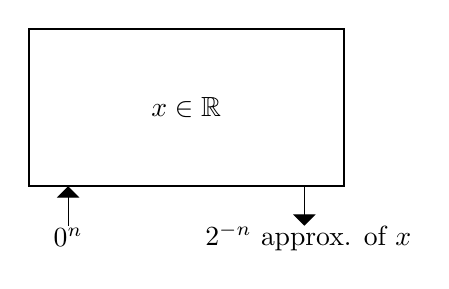
\begin{tikzpicture}
				\path (0,0) rectangle (3.5,-2.7);
			%x
				\draw[thick] (0,0) rectangle (4,-2);
				\node at (2.0,-1) {$x \in \RR$};
				\draw[-triangle 90] (.5,-2.5) -- (.5,-2.0);
				\node at (.5,-2.65) {$0^n$};
				\draw[-triangle 90] (3.5,-2.0) -- (3.5,-2.5);
				\node at (3.55,-2.65) {$2^{-n}$ approx. of $x$};
				%\node<4-> at (2.85,-2.25) {$d_{n,i}$};
				%\node<4-> at (1.5,-1) {$(a_i)$};
				%\draw<4-> (1,-2) -- (1,-2.2);
				%\draw<4->[-triangle 90] (1,-2.5) -- (1,-2.2);
				%\node<4-> at (1.25,-2.25) {$1^i$};
		\end{tikzpicture}
		\end{figure}
\begin{textblock*}{140pt}(10pt,5pt)
  \onslide<2->{
  \begin{tcolorbox}[colback=yellow!5,title={$(\rho_\R^{|[0,1]}, \rho_\R)$-computable},colframe=green!75!black]
    \centering
    \input{computable_rep_fig}
\end{tcolorbox}
    }
  \end{textblock*}
\begin{textblock*}{130pt}(220pt,5pt)
  \onslide<3->{
  \begin{tcolorbox}[colback=yellow!5,title={Computable Function},colframe=red!75!black]
    \centering
    \input{computable_fun_fig}
\end{tcolorbox}
    }
  \end{textblock*}
\end{frame}
\begin{frame}
  \frametitle{Representation for Functions}
  \begin{tcolorbox}[colback=yellow!5,title=Example,colframe=blue!75!black]
    Define a $\delta_\Box$-name of a function $f \in C[0,1]$ as a pair $<\mu, \phi>$ where
    \begin{itemize}
    \item $\mu$ encodes the modulus of continuity (in unary)
    \item $\phi$ is such that $\abs{\phi(d, 0^n)-f(d)} \leq 2^{-n}$ for all $d \in \D \cap [0,1]$
      \end{itemize}
\end{tcolorbox}
\begin{textblock*}{220pt}(140pt,10pt)
  \onslide<2->{
  \begin{tcolorbox}[colback=yellow!5,title=Modulus of Continuity,colframe=red!75!black]
   $\abs{x-y} \leq 2^{-\mu(n)} \Rightarrow \abs{f(x)-f(y)} \leq 2^{-n}$
\end{tcolorbox}
    }
  \end{textblock*}
		\begin{figure}
		\centering
    \vfill
		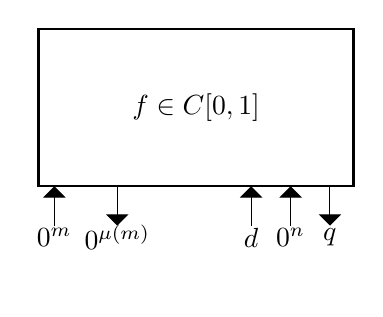
\begin{tikzpicture}
				\path (0,0) rectangle (4.0,-3.3);
			%x
				\draw<3-> [thick] (0,0) rectangle (4,-2);
				\node<3-> at (2.0,-1) {$f \in C[0,1]$};
				\draw<4>[-triangle 90] (.2,-2.5) -- (.2,-2.0);
				\node<4> at (.2,-2.65) {$0^m$};
				\draw<4>[-triangle 90] (1.0,-2.0) -- (1.0,-2.5);
				\node<4> at (1.0,-2.65) {$0^{\mu(m)}$};
				\draw<5>[-triangle 90] (2.7,-2.5) -- (2.7,-2.0);
				\node<5> at (2.7,-2.65) {$d$};
				\draw<5>[-triangle 90] (3.2,-2.5) -- (3.2,-2.0);
				\node<5> at (3.2,-2.65) {$0^n$};
				\draw<5>[-triangle 90] (3.7,-2.0) -- (3.7,-2.5);
				\node<5> at (3.7,-2.65) {$q$};
				%\node<4-> at (2.85,-2.25) {$d_{n,i}$};
				%\node<4-> at (1.5,-1) {$(a_i)$};
				%\draw<4-> (1,-2) -- (1,-2.2);
				%\draw<4->[-triangle 90] (1,-2.5) -- (1,-2.2);
				%\node<4-> at (1.25,-2.25) {$1^i$};
		\end{tikzpicture}
		\end{figure}
                
  \end{frame}
\begin{frame}
  \frametitle{Type-2 Complexity Theory}
  \begin{itemize}
  \item<1-> Let $\sigmas$ be the set of length-monotone string-functions % , i.e. s.t. $\abs{x} \leq \abs{y} \Rightarrow \abs{\varphi(x)} \leq \abs{\varphi(y)}$.
  \item<2-> Define $\abs{\varphi} : \N \to \N$ by $\abs{\varphi}(\abs{u}) = \abs{\varphi(u)}$
   \item<3-> Bound running time by second order polynomials $P(\abs{\varphi})(\abs{x})$
   \item<5->  Can define complexity classes \fpt, \sharpt and \fpspacet 
   \item<6->  Can also define complexity classes \pt, \npt and \pspacet by considering functions $\varphi : \sigmas \to (\Sigma^* \to \{0,1\})$
     \item<7-> Type-2 classes are easy to seperate
  \end{itemize}
\begin{textblock*}{310pt}(50pt,10pt)
  \onslide<4>{
  \begin{tcolorbox}[colback=yellow!5,title=Second Order Polynomials,colframe=red!75!black]
    Defined inductively by
    \begin{enumerate}
    \item $P(L,n) := m$, for $m \in \N$ 
    \item $P(L,n) := n$
    \item $P,Q$ second order polynomials $\Rightarrow$ $P+Q$, $P \cdot Q$ 
    \item $P$ a second order polynomial $\Rightarrow$ $L(Q)$ 
   \end{enumerate}
    Example: $P(L,n) = 2L(L(L(n) \cdot L(n)+2L(n))+2)+n+10$
\end{tcolorbox}
    }
  \end{textblock*}
\end{frame}
\section{Small Complexity Classes}
\subsection*{Definition}
\begin{frame}
  \frametitle{Small Complexity Classes}
  \centering
  \foreach \x in {1,...,3} {
    \only<\x>{
      \includesvg[width=1.1\textwidth]{complexity\x}
    }
  }
\end{frame}
\begin{frame}
  \frametitle{Small Complexity Classes}
  \centering
  \foreach \x in {1,...,5} {
    \only<\x>{
      \includesvg[width=1.0\textwidth]{logspace\x}
    }
  }
\end{frame}
%% \begin{frame}
%%  \frametitle{Logspace Computability} 
%%  For logspace-computability we want the space the machine uses to be bound by $\log(P(\abs{\phi})(\abs{u}))$.\\
%%  (Read-only) input and (write-only) output tapes do not count towards the space-bound.\\ 
%%  What about the query tape?\\
%%  \pause
%%  The machine needs to be able to make queries of polynomial length - otherwise only constant functions can be computed.\\
%%  \pause
%%  Ko defines logarithmic-space computable real-functions by not counting the query and answer tapes towards the space limit.\\
%%  This works for when only dealing with queries of the form $0^n$ but for general oracle functions $\phi$ it would allow iterating the function $\phi$ polynomially many times.
%% \end{frame}
\begin{frame}
\frametitle{The stack model (Kawamura and Ota)}
  \centering
  \foreach \x in {1,...,5} {
    \only<\x>{
      \includesvg[width=1.0\textwidth]{stackmodel\x}
    }
    }
\end{frame}
\begin{frame}
  \frametitle{Example}

\pgfdeclarelayer{background}
\pgfdeclarelayer{foreground}
    \pgfsetlayers{background,main,foreground}
\begin{pgfonlayer}{foreground}
        
\begin{tikzpicture}[remember picture,overlay]
\node<2-12>[draw,line width=2pt,magenta,circle,fit={([yshift=1pt]pic cs:startdb) ([yshift=1pt]pic cs:enddb)}] (n1) {};
\node<3-12>[draw,line width=2pt,red,ellipse,inner ysep=9pt,fit={([yshift=1pt,xshift=14pt]pic cs:startr1) ([yshift=1pt,xshift=-14pt]pic cs:endr2)}] (n2) {};
\end{tikzpicture}  
\begin{tikzpicture}[remember picture,overlay]   %% use here too
        \path[draw=magenta,line width=3pt,->]<2-12> ([yshift=-0.5mm,xshift=0mm]n1.north) to [out=0, in=0,distance=-0.2in] ([yshift=-3mm]t1.west);
\end{tikzpicture}
\begin{tikzpicture}[remember picture,overlay]   %% use here too
        \path[draw=red,line width=3pt,->]<3-12> ([yshift=-0.5mm,xshift=0mm]n2.north) to [out=0, in=0,distance=0.0in] ([yshift=4mm,xshift=-7mm]t2.west);
\end{tikzpicture}
  \end{pgfonlayer}
\begin{textblock*}{120pt}(10pt,2pt)
\onslide<2-12>{
  \begin{tcolorbox}[colback=yellow!5,colframe=magenta!75!black]
		\begin{figure}
		\centering
		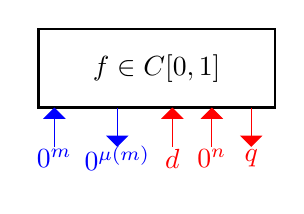
\begin{tikzpicture}[remember picture]
				\path (0,0) rectangle (3.0,-2.0);
				\node at (1.5,-0.5) {$f \in C[0,1]$};
				\draw [thick] (0,0) rectangle (3,-1);
				\draw[-triangle 90, blue] (.2,-1.5) -- (.2,-1.0);
				\node[blue] (t1) at (.2,-1.65) {$0^m$};
				\draw[blue, -triangle 90] (1.0,-1.0) -- (1.0,-1.5);
				\node[blue] at (1.0,-1.65) {$0^{\mu(m)}$};
				\draw[red, -triangle 90] (1.7,-1.5) -- (1.7,-1.0);
				\node[red] at (1.7,-1.65) {$d$};
				\draw[-triangle 90, red] (2.2,-1.5) -- (2.2,-1.0);
				\node[red] at (2.2,-1.65) {$0^n$};
				\draw[red, -triangle 90] (2.7,-1.0) -- (2.7,-1.5);
				\node[red] at (2.7,-1.65) {$q$};
		\end{tikzpicture}
		\end{figure}
  \end{tcolorbox}
 }
\end{textblock*}
\begin{textblock*}{90pt}(220pt,2pt)
\onslide<3-12>{
  \begin{tcolorbox}[colback=yellow!5,colframe=red!75!black]
		\begin{figure}
		\centering
		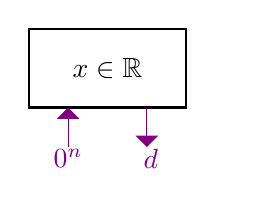
\begin{tikzpicture}[remember picture]
				\path (0,0) rectangle (2.5,-1.7);
			%x
				\draw[thick] (0,0) rectangle (2,-1);
				\node at (1.0,-0.5) {$x \in \RR$};
				\draw[-triangle 90, violet] (.5,-1.5) -- (.5,-1.0);
				\node [violet](t2) at (.5,-1.65) {$0^n$};
				\draw[-triangle 90,violet] (1.5,-1.0) -- (1.5,-1.5);
				\node [violet] at (1.55,-1.65) {$d$};
		\end{tikzpicture}
		\end{figure}
  \end{tcolorbox}
 }
\end{textblock*}
 
\vspace{20pt}
  \begin{tcolorbox}[colback=yellow!5,title=Function Application,colframe=blue!75!black]
    The function $\text{Apply}: C[0,1] \times [0,1] \to \RR,\, (f,x) \mapsto f(x) $ is
    $([\tikzmark{startdb}\delta_\Box\tikzmark{enddb}, \tikzmark{startr1}\rho_\RR^{|[0,1]}]\tikzmark{endr1}, \tikzmark{startr2}\rho_\RR)\tikzmark{endr2}-$FL computable. \\
      %% \tikz[remember picture] \node[coordinate] (n1) {};
\end{tcolorbox}
 \begin{overlayarea}{345pt}{150pt}
   \vfill
\only<4>{
\texttt{
\begin{tabular}{ll}
Input:& $0^n$ \\
Stack:& - \\
Oracle Output:& $\varepsilon$ \\
Work:& $\varepsilon$ \\
Output:& $\varepsilon$ 
\end{tabular}
}
}
\only<5>{
\texttt{
\begin{tabular}{ll}
Input:& $0^n$ \\
Stack:& $\varepsilon$;$\varepsilon$;$\varepsilon$ \\
Oracle Output:& $\varepsilon$ \\
Work:& $\varepsilon$ \\
Output:& $\varepsilon$ 
\end{tabular}
}
}
\only<6>{
\texttt{
\begin{tabular}{ll}
Input:& $0^n$ \\
Stack:& $\textcolor{blue}{0^{n+1}}$;$\varepsilon$;$\varepsilon$ \\
Oracle Output:& $\varepsilon$ \\
Work:& $\varepsilon$ \\
Output:& $\varepsilon$ 
\end{tabular}
}
}
\only<7>{
\texttt{
\begin{tabular}{ll}
Input:& $0^n$ \\
Stack:& $\varepsilon$;$\varepsilon$ \\
Oracle Output:& $\textcolor{blue}{0^m}$ \\
Work:& $\varepsilon$ \\
Output:& $\varepsilon$ 
\end{tabular}
}
\begin{textblock*}{20pt}(150pt,160pt)
\colorbox{yellow}{
$\abs{x-y} \leq 2^{-m} \Rightarrow \abs{f(x)-f(y)} \leq 2^{-(n+1)}$
}
\end{textblock*}
}
\only<8>{
\texttt{
\begin{tabular}{ll}
Input:& $0^n$ \\
Stack:& $\textcolor{violet}{0^{m}}$;$\varepsilon$ \\
Oracle Output:& $\textcolor{blue}{0^m}$ \\
Work:& $\varepsilon$ \\
Output:& $\varepsilon$ 
\end{tabular}
}
}
\only<9>{
\texttt{
\begin{tabular}{ll}
Input:& $0^n$ \\
Stack:& $\varepsilon$ \\
Oracle Output:& $\textcolor{violet}{d}$ \\
Work:& $\varepsilon$ \\
Output:& $\varepsilon$ 
\end{tabular}
}
\begin{textblock*}{20pt}(150pt,160pt)
\colorbox{yellow}{
$\abs{x-d} \leq 2^{-m}$
}
\end{textblock*}
}
\only<10>{
\texttt{
\begin{tabular}{ll}
Input:& $0^n$ \\
Stack:& $\textcolor{red}{d,0^{n+1}}$ \\
Oracle Output:& $\textcolor{violet}{d}$ \\
Work:& $\varepsilon$ \\
Output:& $\varepsilon$ 
\end{tabular}
}
}
\only<11>{
\texttt{
\begin{tabular}{ll}
Input:& $0^n$ \\
Stack:& - \\
Oracle Output:& $\textcolor{red}{q}$ \\
Work:& $\varepsilon$ \\
Output:& $\varepsilon$ 
\end{tabular}
}
\begin{textblock*}{20pt}(150pt,160pt)
\colorbox{yellow}{
$\abs{q-f(d)} \leq 2^{-(n+1)}$
}
\end{textblock*}
}
\only<12>{
\texttt{
\begin{tabular}{ll}
Input:& $0^n$ \\
Stack:& - \\
Oracle Output:& \textcolor{red}{$q$} \\
Work:& $\varepsilon$ \\
Output:& $q$ 
\end{tabular}
}
\begin{textblock*}{20pt}(150pt,190pt)
\colorbox{yellow}{
$\abs{q-f(x)} \leq 2^{-n}$
}
\end{textblock*}
}
\only<13>{
    \begin{tcolorbox}[colback=yellow!5,colframe=red!75!black]
  Similarly, $\text{Apply}^c: C[0,1] \times [0,1] \to [0,1]\,\, (f,x) \mapsto f^c(x) $ is $([\delta_\Box, \rho_\RR^{|[0,1]}], \rho_\RR)-$FL computable for constant $c \in \N$ using a stack of size $2c+1$.
  \end{tcolorbox}
}
\end{overlayarea}
\end{frame}
\section{Analytic Functions}
\subsection{Motivation}
\begin{frame}
\frametitle{Some Results from Real Complexity Theory}
  \begin{tcolorbox}[colback=yellow!5,title=Fact,colframe=blue!75!black]

For general polynomial time computable functions, many important operators have been shown to be computationally hard.\\
For example
\begin{itemize}[<+->]
\item Polynomial time computable functions may have noncomputable derivatives. (Ko 1983)
\item Parametric maximization is NP-hard. (Ko/Friedman (1982))
\item Integration is \#P-hard. (Friedman (1984))
\end{itemize}
\end{tcolorbox}
\end{frame}
\subsection{Complexity for Analytic Functions}
\begin{frame}
\frametitle{Analytic Function}
An analytic function is a function locally given by a complex power series.\\
\begin{definition}[Analytic Function]
$f : D \to \C $, $D \subseteq \C$ is analytic if for any $x_0 \in D$ the Taylor-series
$$ T(x) := \sum^\infty_{n=0} a_n(x-x_0)^n$$
converges to $f(x)$ for $x$ in a neighborhood of $x_0$.  
\end{definition}
\onslide<3>{
\begin{theorem}[Pour-El, Richards, Ko, Friedman, M\"uller (1987/1989)]
$f$ is (polytime) computable iff $(a_m)_{m \in \N}$ is.
\end{theorem}
From that polynomial time computability of the derivative and the anti-derivative of a function follows immediately.
\begin{textblock*}{270pt}(70pt,30pt)
}
\onslide<2->{
  \begin{tcolorbox}[colback=yellow!5,title=Computable Sequence,colframe=green!75!black]
$(a_m)_{m \in \N}$ is computable if there is a machine that on input $1^n, 1^m$ outputs a rational approximation $d_{n,m}$ with $\abs{d_{n,m}-a_m} \leq 2^{-n}$
\end{tcolorbox}
}
\end{textblock*}

\end{frame}
\begin{frame}
\frametitle{Representation for Analytic Functions}
How to represent analytic functions?
\pause
\begin{theorem}[M\"uller (1995)]
The evaluation operator $((a_m)_{m \in \N},x) \to f(x) $ is not computable.
\end{theorem}
\pause
\begin{lemma}
  Let $f : \overline B(0,1) \to \R$ be analytic and $(a_n)_{n \in \N}$ its power series around $0$.\\
  Then there exist $k,A \in \N$ such that 
  \begin{enumerate}
  \item $\sqrt[k]{2}$ is a lower bound on the radius of convergence
  \item $\abs{a_n} \leq A \cdot 2^{-\frac{n}{k}}$
  \end{enumerate}
\end{lemma}
\end{frame}
\begin{frame}
\frametitle{How to represent analytic functions?}
\begin{representation1}
  A function $\varphi \in \sigmas$ is a name for a power series $(a_k)_{k \in \N}$ iff it is a concatenation of the following
  \begin{enumerate}
  \item An integer $A$ encoded in binary
  \item An integer $k$ encoded in unary
  \item A name for a sequence $(a_k)_{k \in \N}$
  \end{enumerate}
  Such that $\abs{a_n} \leq A \cdot 2^{-\frac{n}{k}}$ for all $n \in \N$.
\end{representation1}
\end{frame}
\begin{frame}
\frametitle{How to represent analytic functions?}
\begin{representation2}
  A (length-monotone) function $\varphi: \Sigma^* \to \Sigma^*$ is a name for an analytic function $f:\bar B(0,1) \to \R$ iff it is a concatenation of the following  
  \begin{enumerate}
  \item An integer $A$ encoded in binary,
  \item An integer $k$ encoded in unary,
  \item A name for the function $f$
  \end{enumerate}
  Such that $f$ extends analytically to $B(0, \sqrt[k]{2})$ and $\abs{f(z)} \leq A$ for all $z \in B(0, \sqrt[k]{2})$
\end{representation2}
\end{frame}
\begin{frame}
\frametitle{Analytic Functions and Computational Complexity}
\begin{theorem}[Kawamura, R\"osnick, M\"uller, Ziegler (2013)]
  With the previous two representations the following operations can be performed in polynomial time
\begin{enumerate}
\item evaluation
\item addition and multiplication
\item differentiation and anti-differentiation
\item parametric maximization
\end{enumerate}
\pause
Further, when identifying an analytic function with its power series, the operators that compute one representation from the other are polynomial-time computable.
\end{theorem}
\end{frame}
\begin{frame}
\frametitle{Complexity of Ordinary Differential Equations}
\begin{theorem}[Kawamura, 2010]
Consider the IVP
$$
y'(t)=f(t,y(t)) \quad;\quad y(0)=0.
$$
There exists functions $f: [0,1] \times [-1,1] \to \RR$ and  $y: [0,1] \to [-1,1]$  as above such that
\begin{enumerate}
\item $f$ is Lipschitz-continuous and polynomial time computable
\item $y$ is PSPACE-hard.
\end{enumerate}
\end{theorem}
\pause
  \begin{tcolorbox}[colback=yellow!5,colframe=red!75!black]
    \Large
    For analytic right-hand side the problem can be solved in polynomial time.
    \end{tcolorbox}
\end{frame}
\subsection{Analytic Functions and Small Complexity Classes}
\begin{frame}
\frametitle{Analytic Functions and Small Complexity Classes}
  Consider functions complex analytic on the closed unit disc.
\begin{representation1}
  Integers $A$, $k$ and the series sequence $(a_k)_{k \in \N}$.\\
  $\abs{a_n} \leq A \cdot 2^{-\frac{n}{k}}$ for all $n \in \N$.
\end{representation1}
\begin{representation2}
  Integers $A$, $k$, and name for function $f$.\\
  $f$ extends analytically to $B(0, \sqrt[k]{2})$ and $\abs{f(z)} \leq A$ for all $z \in B(0, \sqrt[k]{2})$
\end{representation2}
Those two representations are logspace equivalent.
\end{frame}
\begin{frame}
\frametitle{Representation 1 $\Rightarrow$ Representation 2}
Given $A$, $k$ s.t. 
  $\abs{a_n} \leq A \cdot 2^{-\frac{n}{k}} \text{ for all } n \in \N.$
Need $A'$, $k'$ s.t. for all $z \in B(0, \sqrt[k']{2})$
$\abs{f(z)} \leq A'$\\
\vfill
\pause
Let $k' = 2k$ and $A' = 4kA$ \\
For $z \in B(0, \sqrt[k']{2})$
$$f(z) = \sum_{n=0}^\infty a_nz^n \leq A\sum_{n=0}^\infty 2^{-\frac{n}{k}} \cdot 2^{\frac{n}{2k}} \leq 4Ak$$
\end{frame}
\begin{frame}
\frametitle{Representation 1 $\Rightarrow$ Representation 2}
$n \mapsto n+\log_2(A)+2\log_2(k)+5$ is a modulus of continuity for the function.\\
\pause
Further, we need to evaluate the function.\\
Note that the following is logspace computable 
\begin{enumerate}[<+->]
\item Addition of polynomially (in $n$) many $n$-bit integers
\item Multiplication of polynomially (in $n$) many $n$-bit integers
\item Compute $x^m$ with precision polynomial in $n$ where $m$ is an integer of length polynomial in $n$
 \item Composition of a constant number of logspace computable functions
\end{enumerate}
\pause
Thus $\sum_{j=0}^{poly(n)} a_jx^j$ is logspace computable.\\
We need to evaluate $N \approx n \cdot k + \log(A)$ terms.
\end{frame}
\begin{frame}
\frametitle{Analytic Functions and Small Complexity Classes}
  Consider functions complex analytic on the closed unit disc.
\begin{representation1}
  Integers $A$, $k$ and the series sequence $(a_k)_{k \in \N}$.\\
  $\abs{a_n} \leq A \cdot 2^{-\frac{n}{k}}$ for all $n \in \N$.
\end{representation1}
\begin{representation2}
  Integers $A$, $k$, and name for function $f$.\\
  $f$ extends analytically to $B(0, \sqrt[k]{2})$ and $\abs{f(z)} \leq A$ for all $z \in B(0, \sqrt[k]{2})$
\end{representation2}
Those two representations are logspace equivalent.
\end{frame}
\begin{frame}
\frametitle{Representation 2 $\Rightarrow$ Representation 1}
Given $A$, $k$ s.t. for all $z \in B(0, \sqrt[k']{2})$
$\abs{f(z)} \leq A$\\
\pause
Need $A'$, $k'$ such that $\abs{a_m} \leq A \cdot 2^{-\frac{m}{k}} \text{ for all } m \in \N.$\\
\pause
By Cauchy's integral formula $\abs{a_m} = \frac{f^{(m)}(0)}{m!} \leq A \cdot 2^{-\frac{n}{k}}$ for all $n \in \N$. \\
Thus, we can just set $A' = A$ and $k' = k$.\\
\pause
Further we need to compute the coefficients for the power series around $0$.\\
\begin{itemize}[<+->]
\item Approximating the derivatives can be done by first approximating the function by a polynomial and then differentiating this polynomial (M\"{u}ller).
\item To get the coefficient $a_m$  the function has to be evaluated at $2m+1$ equidistant points with polynomial precision.
\item Note that Computing factorials and binomial coefficients of polynomial size is logspace computable.
\end{itemize}
\end{frame}
\begin{frame}
\frametitle{Further Operations}
  \begin{tcolorbox}[colback=yellow!5,title=Logspace computable operations,colframe=blue!75!black]

  Similarly, the following operations on analytic functions are computable in logartihmic-space
  \begin{enumerate}[<+->]
    \item Addition, Subtraction, Multiplication of two analytic functions
    \item Computing the $d$-fold derivative
    \item Computing the $d$-fold anti-derivative
   \end{enumerate}
  \end{tcolorbox}
\end{frame}
\subsection{Multidimensional analytic functions}
\begin{frame}
  \frametitle{Multidimensional Analytic Functions}
  \begin{tcolorbox}[colback=yellow!5,title=Multidimensional Power Series,colframe=green!75!black]
    \begin{eqnarray*}
      \sum_{i \in \N} \sum_{j \in \N} a_{i,j} x_1^{i} x_2^{j} & = & \sum_{i \in \N} b_i x_1^{i} \\
      \text{with }
      b_i &:=& \sum_{j \in \N} a_{i,j}x_2^j
    \end{eqnarray*}
    Computing $b_i \rightarrow $ evaluating an analytic function.
\end{tcolorbox}
  \pause
  $\abs{a_{i,j}} \leq A \cdot 2^{-\frac{i+j}{k}}$ for all $n \in \N$. \\
  $\abs{b_i} \leq \sum_{j \in \N} \abs{a_{i,j}}\abs{x_2}^j \leq A2^{-\frac{i}{k}} \sum_{j \in \N} 2^{-\frac{j}{k}} = A2^{-\frac{j}{k}}\frac{\sqrt[k]{2}}{\sqrt[k]{2}-1} \leq \textbf{(2Ak)}2^{-\frac{i}{k}}   $
  \end{frame}
\begin{frame}
  \frametitle{Multidimensional analytic functions}
   \begin{tcolorbox}[colback=yellow!5,title=Representation,colframe=blue!75!black]
  A function $\varphi \in \sigmas$ is a name for a $d$ dimensional power series $(a_{n_1,\dots,n_d})_{n_1,\dots,n_d \in \N}$ iff it is a concatenation of the following
  \begin{enumerate}
  \item An integer $A$ encoded in binary
  \item An integer $k$ encoded in unary
  \item A name for a sequence $(a_k)_{k \in \N}$
  \end{enumerate}
  Such that $\abs{a_{n_1,\dots,n_d}} \leq A \cdot 2^{-\frac{n_1+\dots+n_d}{k}}$ for all $n \in \N$.
\end{tcolorbox}
   \pause
  \begin{tcolorbox}[colback=yellow!5,title=Note,colframe=red!75!black]
    Complexity of evaluation (and most other operations) is \textbf{exponential} in the dimension!
  \end{tcolorbox}
  \end{frame}
\begin{frame}
  \frametitle{Future Work: P-completeness}
  Kawamura and Ota also define the notions of reductions and completeness.
  \pause
  For example they give the following uniform version of a theorem by Ko
  \begin{theorem}
    For the set $M$ of bijective functions in $C[0,1]$, define the $\delta_{\Box INV}$ representation by adding a modulus of continuity for the inverse function to the $\delta_{\Box}$ representation.\\
    The function $Inv: M \to C[0,1],\, Inv(f) \mapsto f^{-1}$ is $(\delta_{\Box INV}, \delta_{\Box})$-FP-complete.
  \end{theorem}
  \pause
  Which operations on analytic functions are P-hard?
  \begin{itemize}
  \item Initial Value Problem?
    \item Maximization?
    \end{itemize}
\end{frame}
\begin{frame}
  \frametitle{Future Work: P-completeness}
\end{frame}
\subsection*{Overview and Future Work}
\begin{frame}
  \frametitle{Conclusion}
  \begin{itemize}
    \item Presented Kawamura and Ota's model for logspace computability in analysis.
    \item In this model many operations on analytic functions are logspace computable, when considering representations that have previously been considered for polynomial time computability.
    \item Open Problems: Parametrized Maximization, Ordinary Differential Equations
     \item Connection to parallelization in exact real arithmetic
     \item Implementations
  \end{itemize}
\end{frame}
\end{document}
